%!TEX options = -shell-escape

\documentclass[glossy]{beamer}

% Fonts
\usepackage[utf8]{inputenc}
\usepackage{lmodern}
\usepackage[T1]{fontenc}

% Beamer
\useoutertheme{wuerzburg}
\useinnertheme[realshadow,corners=2pt,padding=2pt]{chamfered}
\usecolortheme{shark}

\setbeamertemplate{navigation symbols}{}

% Tikz
\usepackage{tikz}
\usetikzlibrary{tikzmark, arrows, decorations, decorations.pathreplacing}
\tikzset{every picture/.style={font issue=\scriptsize},
         font issue/.style={execute at begin picture={#1\selectfont}}
}

\tikzstyle{callout}=[remember picture, ->, >=stealth, overlay, red, ultra thick, align=center, anchor=west]

% Minted
\usepackage{minted}
\newminted{cpp}{autogobble, fontsize=\tiny, escapeinside=@@}
\newmintedfile{cpp}{autogobble, fontsize=\tiny, escapeinside=@@}
\newmintinline{cpp}{escapeinside=@@}
\newmintinline{java}{}
\newmintinline{js}{}
\usemintedstyle{vs}

% GraphicX
\usepackage{graphicx}
\graphicspath{{img/}}

% Macros
\newcommand{\cppref}[2]{\href{http://en.cppreference.com/w/cpp/#1}{\underline{#2}}}
\newcommand{\refer}[1]{([shift={(.25em,.25em)}]pic cs:#1)}

% Meta
\title{C++ Boot Camp 1/2}
\author{Jesse Talavera-Greenberg}
\date{}

\begin{document}

\begin{frame}[fragile=singleslide]
  \frametitle{C++ Boot Camp 1/2}
  \framesubtitle{Jesse Talavera-Greenberg}
  \begin{figure}
    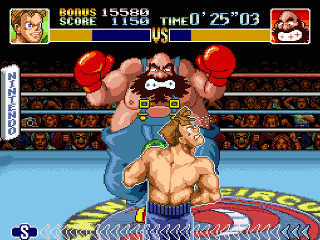
\includegraphics[width=.75\columnwidth]{super-punch-out}
    \centering
  \end{figure}
  \begin{tikzpicture}[callout, line width=2mm]
    \draw (3.5cm, 2cm) node [anchor=east] {\huge \textbf{You}} -> (6.25cm, 3.5cm);
    \draw (8.5cm, 5.75cm) node  {\huge \textbf{C++}} -> (6.5cm, 5.5cm);
  \end{tikzpicture}
\end{frame}

%%%%%%%%%%%%%%%%%%%%%%%%%%%%%%%%%%%%%%%%%%%%%%%%%%%%%%%%%%%%%%%%%%%%%%%%%%%%%%%

\begin{frame}[fragile=singleslide]
  \frametitle{Disclaimers}
  \begin{itemize}
    \item I am not the grader for this course.
    \item This boot camp is entirely voluntary.
    \item Any opinions expressed are my own.
    \item I don't know much about DirectX.
    \item Correctness is likely, but \textbf{not guaranteed}.
  \end{itemize}
\end{frame}

%%%%%%%%%%%%%%%%%%%%%%%%%%%%%%%%%%%%%%%%%%%%%%%%%%%%%%%%%%%%%%%%%%%%%%%%%%%%%%%

\begin{frame}[fragile=singleslide]
  \frametitle{Not Your Daddy's Programming Language}
  \begin{columns}
    \begin{column}{6cm}
      \begin{itemize}
        \item Originally designed for C compatibility
        \item High-level abstractions
        \item Low-level resource management
        \item OOP is entirely optional
        \item Follow along in-browser on \href{http://coliru.stacked-crooked.com/}{Coliru} and \href{http://www.cppreference.com}{cppreference.com}
      \end{itemize}
    \end{column}

    \begin{column}{6cm}
      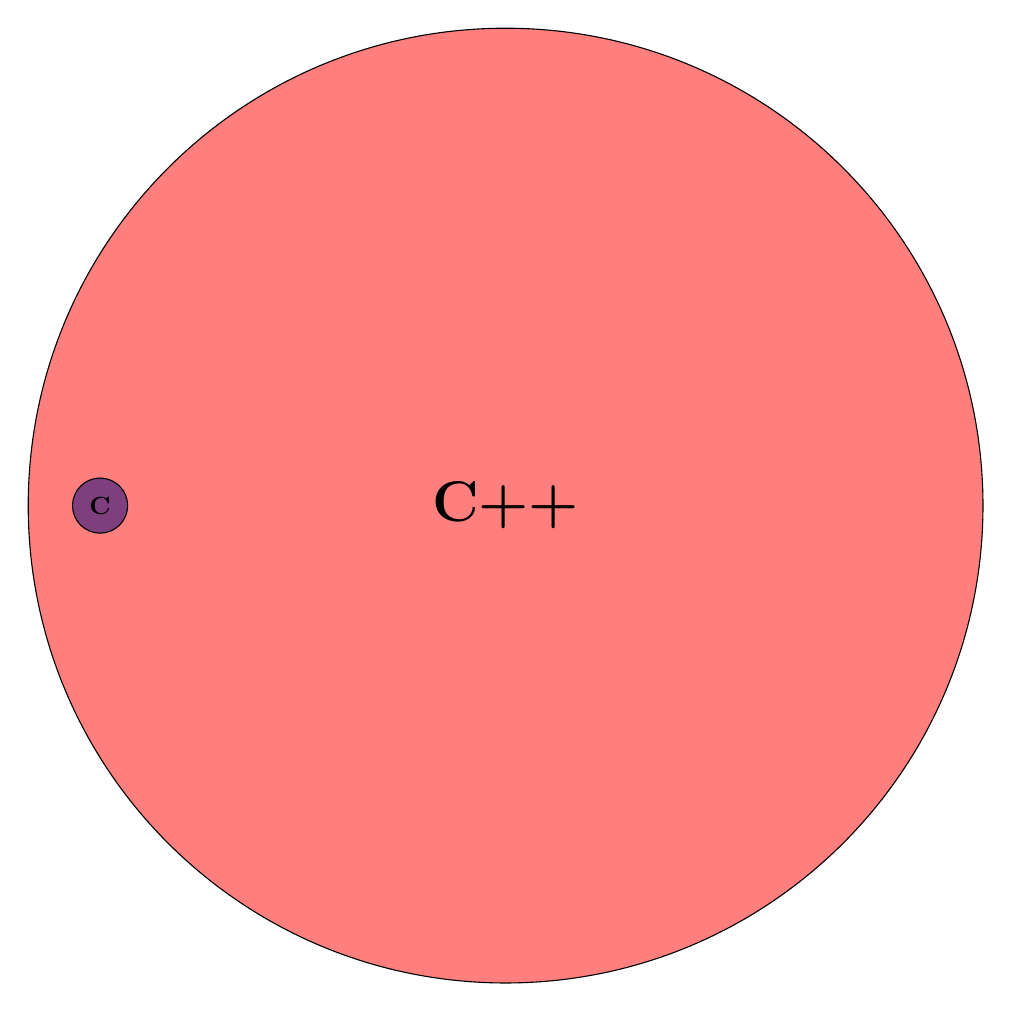
\begin{tikzpicture}[align=center, blend mode=multiply, anchor=center]
        \draw [fill=red, fill opacity=0.5] (0.4\columnwidth,8) circle (0.5\columnwidth) node [fill opacity=1] {\huge{\textbf{C++}}};
        \draw [fill=blue, fill opacity=0.5] (-0.3,8) circle (.35cm) node [fill opacity=1] {\small{\textbf{C}}};
      \end{tikzpicture}
    \end{column}
  \end{columns}
\end{frame}

%%%%%%%%%%%%%%%%%%%%%%%%%%%%%%%%%%%%%%%%%%%%%%%%%%%%%%%%%%%%%%%%%%%%%%%%%%%%%%%

\begin{frame}[fragile=singleslide]
  \frametitle{\cppref{language/basic_concepts}{The Basics}}

  \cppfile{src/basic.cpp}
  
  
\begin{tikzpicture}[callout]
    \draw (4.5cm, 26em) node  {\cppref{preprocessor/include}{Enable functionality}} -> \refer{basic_include};
    \draw (7cm, 24em) node  {\# of command-line arguments} -> \refer{basic_argc};
    \draw (7cm, 21em) node  {Actual arguments} -> \refer{basic_argv};
    \draw[decorate, decoration={brace}, -] ({pic cs:basic_using_a} |- {pic cs:basic_using_b}) +(0,1.5em) -- node [right, inner sep=1em] {Pulls into namespace\\(avoid long-ass prefixes)} ({pic cs:basic_using_a} |- {pic cs:basic_using_b});
    \draw (7cm, 15em) node  {\cppref{io}{Formatted printout}} -> \refer{basic_print};
    \draw (5cm, 3em) node  {Return code (absence in \verb|main| implies 0)} -> \refer{basic_return};
    \draw (4cm, 12em) node  {Strings not allowed\\in \verb|switch| statements} -> \refer{basic_switch};
  \end{tikzpicture}
\end{frame}

%%%%%%%%%%%%%%%%%%%%%%%%%%%%%%%%%%%%%%%%%%%%%%%%%%%%%%%%%%%%%%%%%%%%%%%%%%%%%%%

\begin{frame}[fragile=singleslide]
  \frametitle{\cppref{language/types}{Fundamental Types}}
  \begin{columns}[t]
    \begin{column}{6cm}
      \begin{itemize}
        \item Integer sizes \cppref{language/types\#Data_models}{\textbf{can vary}} by platform, compiler, and OS
        \item No \javainline|byte| (use \cppinline|uint8_t|)
        \item \javainline|boolean| $\rightarrow$ \cppref{language/types\#Boolean_type}{\cppinline|bool|}
        \item Numbers \cppref{language/implicit_cast}{implicitly cast} to \cppinline|bool|
        \item Use \cppref{language/nullptr}{\cppinline|nullptr|} for null pointers, not \javainline|null| or \cppref{types/NULL}{\cppinline|NULL|}
        \item \cppinline|float| and \cppinline|double| exist (also \cppinline|long double|)
      \end{itemize}
    \end{column}

    \begin{column}{6cm}
      \begin{itemize}
        \item \cppinline|unsigned|s can't be negative
        \item For specific sizes, \cppinline|#include @\cppref{preprocessor/include}{<cstdint>}@| and use \jsinline{/std::u?int(8|16|32|64)_t/}
        \item There is \textbf{no} root object class
      \end{itemize}
    \end{column}
  \end{columns}
\end{frame}

%%%%%%%%%%%%%%%%%%%%%%%%%%%%%%%%%%%%%%%%%%%%%%%%%%%%%%%%%%%%%%%%%%%%%%%%%%%%%%%

\begin{frame}[fragile=singleslide]
  \frametitle{\cppref{language/exceptions}{Exceptions}}
  
  \cppfile{src/exception.cpp}

  \begin{tikzpicture}[callout]
    \draw (4cm, 24em) node  {Contains exception-handling functionality} -> \refer{except_header};
    \draw (5cm, 15em) node  {\cppref{language/noexcept_spec}{"I promise not to throw an exception"}} -> \refer{except_noexcept};
    \draw (5cm, 9em) node  {Base exception type} -> \refer{except_type};
    \draw (6cm, 4em) node  {No \verb|finally| statement\\(use \cppref{language/destructor}{destructors} instead)} -> \refer{except_nofinally};
  \end{tikzpicture}
\end{frame}

%%%%%%%%%%%%%%%%%%%%%%%%%%%%%%%%%%%%%%%%%%%%%%%%%%%%%%%%%%%%%%%%%%%%%%%%%%%%%%%

\begin{frame}[fragile=singleslide]
  \frametitle{\cppref{language/type_alias}{Type Aliases}}

  \cppfile{src/typedef.cpp}

  
\begin{tikzpicture}[callout]
    \draw (4cm, 22em) node  {For the \verb|typeid| operator} -> \refer{typedef_typeinfo};
    \draw (3cm, 10.5em) node  {Same type, different names} -> \refer{typedef_okay_a};
    \draw (3cm, 10.5em) -> \refer{typedef_okay_b};
    \draw (6cm, 16em) node  {Prefer \verb|using|, but recognize \verb|typedef|} -> \refer{typedef_prefer};
    \draw (10cm, 11em) node [anchor=south] {Both strings are the same\\(but implementation-defined)} -> \refer{typedef_same_a};
    \draw (10cm, 11em) -> \refer{typedef_same_b};
    \draw (6cm, 19em) node  {Another name for\\the same type} -> \refer{typedef_using_a};
    \draw (6cm, 19em) -> \refer{typedef_using_b};
  \end{tikzpicture}
\end{frame}

%%%%%%%%%%%%%%%%%%%%%%%%%%%%%%%%%%%%%%%%%%%%%%%%%%%%%%%%%%%%%%%%%%%%%%%%%%%%%%%

\begin{frame}[fragile=singleslide]
  \frametitle{A Common Memory Model}
  \begin{columns}
    \begin{column}{6cm}
      \begin{itemize}
        \item Stack is fast, but size must be known at compile time
        \item Heap is flexible, but slow
        \item Details vary by compiler, OS, and hardware
        \item \textbf{All objects of a given type are the same size}
      \end{itemize}
    \end{column}

    \begin{column}{6cm}
      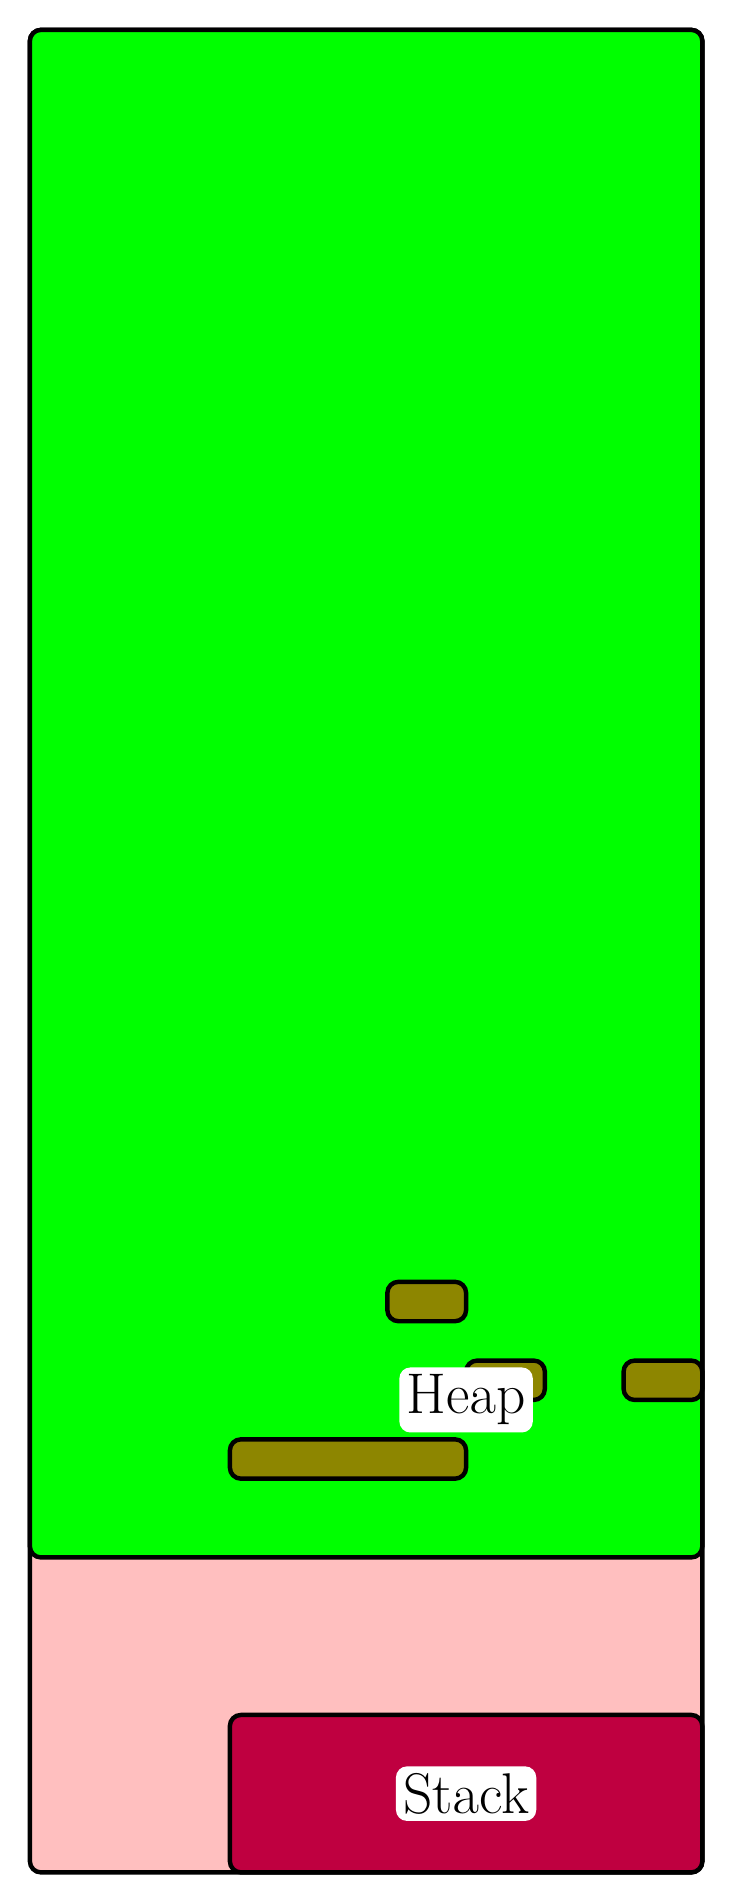
\begin{tikzpicture}[ultra thick, rounded corners]
        \draw [fill=pink] (current page.north west) rectangle (6cm, 2cm);
        \draw [fill=purple] (0cm, 2cm) rectangle (6cm, 4cm) node [align=center, anchor=center, fill=white] at (3cm, 3cm) {\huge{Stack}};
        \draw [fill=green] (current page.north west) rectangle (6cm, 6cm);
        \draw [fill=olive] (2cm, 9cm) rectangle +(1cm, 0.5cm) (3cm, 8cm) rectangle +(1cm, 0.5cm) (5cm, 8cm) rectangle +(1cm, 0.5cm) (0, 7cm) rectangle +(3cm, 0.5cm);
        \draw node [align=center, anchor=center, fill=white] at (3cm, 8cm) {\huge{Heap}};
      \end{tikzpicture}
    \end{column}
  \end{columns}

  \begin{tikzpicture}[callout]
    \draw (4cm, 22em) node [anchor=east] {Find enough space (expensive)} -> (6.25cm, 5.25cm);
    \draw (4cm, 3em) node [anchor=east] {Increment an address (cheap)} -> (6.25cm, 2cm);
  \end{tikzpicture}
\end{frame}

%%%%%%%%%%%%%%%%%%%%%%%%%%%%%%%%%%%%%%%%%%%%%%%%%%%%%%%%%%%%%%%%%%%%%%%%%%%%%%%

\begin{frame}[fragile=singleslide]
  \frametitle{\cppref{language/scope}{Scope} and \cppref{language/lifetime}{Lifetime} (cont'd)}
  \begin{columns}
    \begin{column}{6cm}
      \begin{itemize}
        \item \textbf{static:} Exists for program duration (on stack or in program data)\tikzmark{memory_static_a}
        \item \textbf{automatic:} Disappears when out of scope (on stack)\tikzmark{memory_auto_a}
        \item \textbf{dynamic:} Created and destroyed at will (on heap)\tikzmark{memory_dynamic_a}
        \begin{itemize}
          \item Use one \cppinline{delete} for every \cppinline{new}
          \item Or avoid \cppinline{new} entirely (better)
        \end{itemize}
      \end{itemize}
    \end{column}

    \begin{column}{6cm}
      \cppfile{src/memory.cpp}
    \end{column}
  \end{columns}

  
\begin{tikzpicture}[callout]
    \draw (pic cs:memory_static_a) -> \refer{memory_static_b};
    \draw (pic cs:memory_auto_a) -> \refer{memory_auto_b};
    \draw (pic cs:memory_dynamic_a) -> \refer{memory_dynamic_b};
    \draw (pic cs:memory_dynamic_a) -> \refer{memory_dynamic_c};
  \end{tikzpicture}
\end{frame}

%%%%%%%%%%%%%%%%%%%%%%%%%%%%%%%%%%%%%%%%%%%%%%%%%%%%%%%%%%%%%%%%%%%%%%%%%%%%%%%

\begin{frame}[fragile=singleslide]
  \frametitle{\cppref{language/pointer}{Pointers} Vs. \cppref{language/reference}{References}}

  \begin{itemize}
    \item Access data from multiple places without copying it
    \item Left dangling (\textbf{invalid}) if the underlying object dies
    \begin{itemize}
      \item No way to check for this
      \item Will likely crash if you try to use it
    \end{itemize}
    \item Polymorphism okay
    \item Both compile to similar machine code
  \end{itemize}

  \begin{columns}
    \begin{column}{6cm}
      \textbf{Pointers:}
      \begin{itemize}
        \item May be invalid (dangling)
        \item Can represent lack of data
        \item Syntax to use and declare
        \item Address can be reassigned
      \end{itemize}
    \end{column}

    \begin{column}{6cm}
      \textbf{References:}
      \begin{itemize}
        \item Always initialized
        \item Points to \textbf{exactly one} address
        \item Less syntax
        \item Easier to deal with objects that shouldn't change
      \end{itemize}
    \end{column}
  \end{columns}
\end{frame}

%%%%%%%%%%%%%%%%%%%%%%%%%%%%%%%%%%%%%%%%%%%%%%%%%%%%%%%%%%%%%%%%%%%%%%%%%%%%%%%

\begin{frame}[fragile=singleslide]
  \frametitle{\cppref{language/pointer}{Pointers} Vs. \cppref{language/reference}{References} (cont'd)}
  \begin{columns}[t]
    \begin{column}{6cm}
      \textbf{Pointers:}
      \cppfile{src/pointers.cpp}
    \end{column}

    \begin{column}{6cm}
      \textbf{References:}
      \cppfile{src/references.cpp}
    \end{column}
  \end{columns}
\end{frame}

%%%%%%%%%%%%%%%%%%%%%%%%%%%%%%%%%%%%%%%%%%%%%%%%%%%%%%%%%%%%%%%%%%%%%%%%%%%%%%%

\begin{frame}[fragile=singleslide]
  \frametitle{\cppref{language/ub}{Undefined Behavior}}
  \begin{columns}
    \begin{column}{6cm}
      \begin{itemize}
        \item Java fully defines everything
        \item C++ leaves certain edge cases up to the compiler
        \item Many, many ways to invoke
        \item \textbf{Do not rely on UB}
        \begin{itemize}
          \item Best case scenario: Crash
          \item Worst case scenario: No crash
        \end{itemize}
        \item Distinct from unspecified or implementation-defined behavior
      \end{itemize}
    \end{column}

    \begin{column}{6cm}
      \cppfile{src/ub.cpp}
    \end{column}
  \end{columns}
\end{frame}

%%%%%%%%%%%%%%%%%%%%%%%%%%%%%%%%%%%%%%%%%%%%%%%%%%%%%%%%%%%%%%%%%%%%%%%%%%%%%%%

\begin{frame}[fragile=singleslide]
  \frametitle{\cppref{language/namespace}{Namespaces}}

  \cppfile{src/namespace.cpp}

  
\begin{tikzpicture}[callout]
    \draw (6cm, 22em) node  {Don't do this (or \verb|java.util.*|)} -> \refer{namespace_std};
    \draw (5cm, 19em) node  {Nest them as much as you'd like} -> \refer{namespace_nest_a};
    \draw (5cm, 19em) -> \refer{namespace_nest_b};
    \draw (5cm, 19em) -> \refer{namespace_nest_c};
    \draw (5cm, 8em) node  {Fully-qualified name} -> \refer{namespace_qualified};
    \draw (6cm, 4em) node  {Introduced name} -> \refer{namespace_using};
  \end{tikzpicture}
\end{frame}

%%%%%%%%%%%%%%%%%%%%%%%%%%%%%%%%%%%%%%%%%%%%%%%%%%%%%%%%%%%%%%%%%%%%%%%%%%%%%%%

\begin{frame}[fragile=singleslide]
  \frametitle{\cppref{preprocessor}{The Preprocessor}}

  \cppfile{src/cpp.cpp}

  
\begin{tikzpicture}[callout]
    \draw (3cm, 25em) node  {Use \verb|<>| for libraries, \verb|""| for your code} -> \refer{cpp_include};
    \draw (4cm, 21em) node  {\verb|#define|s can be added by the build process} -> \refer{cpp_define};
    \draw (3cm, 18em) node  {Uncomment these} -> \refer{cpp_windows};
    \draw (3cm, 18em) -> \refer{cpp_mac};
    \draw (4cm, 9em) node  {Contents ignored (not compiled) if on Linux} -> \refer{cpp_linux};
    \draw (5cm, 3em) node  {Intentional compiler error} -> \refer{cpp_error};
  \end{tikzpicture}
\end{frame}

%%%%%%%%%%%%%%%%%%%%%%%%%%%%%%%%%%%%%%%%%%%%%%%%%%%%%%%%%%%%%%%%%%%%%%%%%%%%%%%

\begin{frame}[fragile=singleslide]
  \frametitle{\cppref{language/enum}{Enumerations}}

  \cppfile{src/enum.cpp}

  
\begin{tikzpicture}[callout]
    \draw (3cm, 25em) node  {Scoped \verb|int|s, not objects} -> \refer{enum_not_object};
    \draw (3cm, 22em) node  {Trailing comma OK} -> \refer{enum_comma};
    \draw (3cm, 17em) node  {OK to assign values} -> \refer{enum_value};
    \draw (3cm, 13em) node  {Old-style \verb|enum|s\\(recognize, but avoid)} -> \refer{enum_old};
    \draw (5cm, 8em) node  {Scoped \verb|enum| usage} -> \refer{enum_scoped_a};
    \draw (5cm, 8em) -> \refer{enum_scoped_b};
    \draw (5cm, 5em) node  {Avoid if \verb|enum| is not contiguous} -> \refer{enum_ub};
    \draw (4cm, 3em) node  {Explicitly convert \verb|enum| to \verb|int|} -> \refer{enum_int};
  \end{tikzpicture}
\end{frame}

%%%%%%%%%%%%%%%%%%%%%%%%%%%%%%%%%%%%%%%%%%%%%%%%%%%%%%%%%%%%%%%%%%%%%%%%%%%%%%%

\begin{frame}[fragile=singleslide]
  \frametitle{\cppref{language/classes}{Declaring Classes}}

  \cppfile{src/class.cpp}

  \begin{tikzpicture}[callout]
    \draw (3cm, 17em) node  {\textbf{REQUIRED} for base classes} -> \refer{class_virtual_dtor};
    \draw (3cm, 24em) node  {\cppref{language/access}{Access modifiers same as in Java} (but no package-private)} -> \refer{class_access_a};
    \draw (4cm, 12em) node  {\verb|struct| defaults to \verb|public|\\\verb|class| defaults to \verb|private|} -> \refer{class_struct};
    \draw (2cm, 14em) node  {Remember the semicolon!} -> \refer{class_semicolon};
    \draw (3cm, 22em) node  {\cppref{language/virtual}{Allows method to be overridden}} -> \refer{class_virtual};
    \draw (9cm, 19em) node  {Technically you can,\\but things get weird} -> \refer{class_no_override};
    \draw (2cm, 11em) node [anchor=north] {\cppref{language/abstract_class}{Abstract method}} -> \refer{class_abstract};
    \draw (6cm, 4em) node [anchor=north west] {\cppref{language/override}{Marks method as an override}} -> \refer{class_override};
    \draw (2cm, 2em) node [anchor=north] {Call parents with \verb|class| name} -> \refer{class_super};
    \draw (7cm, 7em) node  {Inheritance (actually six\\kinds; just use \verb|public|)} -> \refer{class_inheritance};
  \end{tikzpicture}
\end{frame}

%%%%%%%%%%%%%%%%%%%%%%%%%%%%%%%%%%%%%%%%%%%%%%%%%%%%%%%%%%%%%%%%%%%%%%%%%%%%%%%

\begin{frame}[fragile=singleslide]
  \frametitle{(\cppref{language/initializer_list}{Con}|\cppref{language/destructor}{De})structors, \cppref{language/raii}{RAII}, and the \cppref{language/rule_of_three}{Rule of 3}}

  \cppfile{src/raii.cpp}

  \begin{tikzpicture}[callout]
    \draw (4cm, 24em) node  {STL does this better} -> \refer{raii_dont};
    \draw (5cm, 22.5em) node {Member initialization syntax} -> \refer{raii_init};
    \draw (4cm, 27em) node {Don't use these (use \verb|string|)} -> \refer{raii_cstring};
    \draw (4cm, 27em) -> \refer{raii_memcpy};
    \draw (8cm, 21em) node {Other code} -> \refer{raii_ctor};
    \draw (9cm, 7em) node [anchor=north] {Rule of 3: You need to write one,\\you need to write them all} -> \refer{raii_copyctor} node [pos=.5, above, sloped, anchor=north] {\cppref{language/copy_constructor}{Copy constructor}};
    \draw (9cm, 7em) -> \refer{raii_dtor} node [pos=.5, above, sloped, anchor=north] {\cppref{language/destructor}{Destructor}};
    \draw (9cm, 7em) -> \refer{raii_copyeq} node [pos=.5, above, sloped, anchor=north] {\cppref{language/copy_assignment}{Copy assignment}};
    \draw (4.5cm, 3em) node [anchor=north] {RAII: Create in ctor, delete in dtor} -> \refer{raii_dtor_b};
  \end{tikzpicture}
\end{frame}

%%%%%%%%%%%%%%%%%%%%%%%%%%%%%%%%%%%%%%%%%%%%%%%%%%%%%%%%%%%%%%%%%%%%%%%%%%%%%%%

\begin{frame}[fragile=singleslide]
  \frametitle{\cppref{language/cv}{\cppinline{const}}}

  \cppfile{src/const.cpp}

  
\begin{tikzpicture}[callout]
    \draw (9cm, 21em) node  {No side effects\\(aka state changes)} -> \refer{const_nochange};
    \draw (9cm, 18em) node  {Immutable reference\\(no state changes)} -> \refer{const_ref};
    \draw (9cm, 15em) node  {Mutable reference\\(state changes possible)} -> \refer{const_nonconst_ref};
    \draw (8cm, 12em) node  {Side effects} -> \refer{const_nonconst};
    \draw (4cm, 11em) node  {\verb|const|-dodging tricks\\are usually UB} -> \refer{const_ub};
    \draw (8cm, 3em) node  {\verb|const| forbids it} -> \refer{const_no_cat};
    \draw (6cm, 7em) node  {One name, two overloads\\(chosen by compiler)} -> \refer{const_overload_a};
    \draw (6cm, 7em) -> \refer{const_overload_b};
  \end{tikzpicture}
\end{frame}

%%%%%%%%%%%%%%%%%%%%%%%%%%%%%%%%%%%%%%%%%%%%%%%%%%%%%%%%%%%%%%%%%%%%%%%%%%%%%%%

\begin{frame}[fragile=singleslide]
  \frametitle{\cppref{language/function\#Deleted_functions}{Deleted Functions}}

  \cppfile{src/deleted.cpp}

  
\begin{tikzpicture}[callout]
    \draw (8cm, 18em) node  {Forbids this special method\\(compiler error if used)} -> \refer{deleted_a};
    \draw (8cm, 18em) -> \refer{deleted_b};
    \draw (4cm, 14em) node  {Still gotta clean up} -> \refer{deleted_cleanup};
    \draw (4cm, 6em) node  {RAII in action} -> \refer{deleted_should};
  \end{tikzpicture}
\end{frame}

%%%%%%%%%%%%%%%%%%%%%%%%%%%%%%%%%%%%%%%%%%%%%%%%%%%%%%%%%%%%%%%%%%%%%%%%%%%%%%%

\begin{frame}[fragile=singleslide]
  \frametitle{\cppref{memory/unique_ptr}{\cppinline{unique_ptr}}}

  \cppfile{src/unique.cpp}

  
\begin{tikzpicture}[callout]
    \draw (4cm, 20em) node [anchor=south west] {At most one \verb|unique_ptr|\\can manage an address} -> \refer{unique_ptr};
    \draw (8cm, 15em) node [anchor=south] {Use \verb|make_unique|, not existing\\pointers (else you risk double-\verb|delete|s)} -> \refer{unique_multiple};
    \draw (5cm, 8em) node  {Cleaned up with RAII} -> \refer{unique_delete};
  \end{tikzpicture}
\end{frame}

%%%%%%%%%%%%%%%%%%%%%%%%%%%%%%%%%%%%%%%%%%%%%%%%%%%%%%%%%%%%%%%%%%%%%%%%%%%%%%%

\begin{frame}[fragile=singleslide]
  \frametitle{\cppref{language/expressions\#Conversions}{Casting}}

  \cppfile{src/cast.cpp}

  \begin{tikzpicture}[callout]
    \draw (6cm, 21em) node  {Polymorphism must be through\\pointers or references} -> \refer{cast_poly};
    \draw (5cm, 16em) node  {Explicit upcasts rarely necessary} -> \refer{cast_upcast_a};
    \draw (5cm, 16em) -> \refer{cast_upcast_b};
    \draw (6cm, 13.5em) node  {\cppref{language/dynamic_cast}{Runtime type check (slow)}} -> \refer{cast_dynamic};
    \draw (6cm, 12em) node  {\cppref{language/static_cast}{Compile-time type assurance (fast)}} -> \refer{cast_static};
    \draw (6cm, 9em) node  {Pointer to derived (success)} -> \refer{cast_dynamic_pass};
    \draw (6cm, 8em) node  {\verb|nullptr| (failure, \verb|bad_cast| if a reference)} -> \refer{cast_dynamic_fail};
    \draw (6cm, 6em) node  {Pointer to derived (hopefully success?)} -> \refer{cast_static_pass};
    \draw (6cm, 5em) node  {Undefined behavior (hopefully success?)} -> \refer{cast_static_fail};
    \draw (3cm, 2em) node  {You fucked up!} -> \refer{cast_ub};
  \end{tikzpicture}
\end{frame}

%%%%%%%%%%%%%%%%%%%%%%%%%%%%%%%%%%%%%%%%%%%%%%%%%%%%%%%%%%%%%%%%%%%%%%%%%%%%%%%

\begin{frame}[fragile=singleslide]
  \frametitle{\cppref{concept}{Concepts}}

  \begin{itemize}
    \item Named requirements for a type or function
    \begin{itemize}
      \item Kind of like compile-time interfaces
      \item \emph{Usually} implementing certain methods
    \end{itemize}
    \item Types may be used in templates if they do certain things
    \item Future language revisions will integrate them into the syntax
  \end{itemize}

  \textbf{Examples:}
  \begin{itemize}
    \item \cppref{concept/EqualityComparable}{\cppinline{EqualityComparable}} $\rightarrow$ provides \cppinline{operator==} for equality test
    \item \cppref{concept/Container}{\cppinline{Container}} $\rightarrow$ holds objects and manages their memory (via RAII)
    \item \cppref{concept/SequenceContainer}{\cppinline{SequenceContainer}} $\rightarrow$ \cppinline{Container} whose elements are sequential
    \item \cppref{concept/FormattedOutputFunction}{\cppinline{FormattedOutputFunction}} $\rightarrow$ Function that outputs an object to a \cppinline{std::ostream} (like \cppinline{std::cout})
  \end{itemize}
\end{frame}

%%%%%%%%%%%%%%%%%%%%%%%%%%%%%%%%%%%%%%%%%%%%%%%%%%%%%%%%%%%%%%%%%%%%%%%%%%%%%%%

\begin{frame}[fragile=singleslide]
  \frametitle{\cppref{language/templates}{Templates}}

  \cppfile{src/template.cpp}

  
\begin{tikzpicture}[callout]
    \draw (3cm, 25em) node [anchor=south west] {Standard library uses\\LOTS of templates} -> \refer{template_stl};
    \draw (7cm, 22em) node  {Almost anything can be \verb|templated|} -> \refer{template_class} node [pos=.5, above, sloped, anchor=south] {classes};
    \draw (7cm, 22em) -> \refer{template_typedef} node [pos=.5, above, sloped, anchor=north] {\verb|typedef|s};
    \draw (7cm, 22em) -> \refer{template_function} node [pos=.5, above, sloped, anchor=north] {(member )?functions};
    \draw (3cm, 11em) node  {For types that depend on template parameters inside templates} -> \refer{template_depend};
    \draw (6cm, 7em) node  {Three different classes\\and chunks of code} -> \refer{template_diff_a};
    \draw (6cm, 7em) -> \refer{template_diff_b};
    \draw (6cm, 7em) -> \refer{template_diff_c};
    \draw (3cm, 4.5em) node  {Function type parameters can be deduced} -> \refer{template_function_deduce};
    \draw (3cm, 3em) node  {Error: No way to print a \verb|Dummy|} -> \refer{template_no_print};
  \end{tikzpicture}
\end{frame}

%%%%%%%%%%%%%%%%%%%%%%%%%%%%%%%%%%%%%%%%%%%%%%%%%%%%%%%%%%%%%%%%%%%%%%%%%%%%%%%

\begin{frame}[fragile=singleslide]
  \frametitle{\cppref{iterator}{Iterators}}

  \cppfile{src/iterator.cpp}

  
\begin{tikzpicture}[callout]
    \draw (3cm, 13em) node {Deduce the type\\(used for long names)} -> \refer{iterator_auto};
    \draw (8cm, 8em) node {Probably an ordinary pointer\\(but who cares?)} -> \refer{iterator_ptr};
    \draw (5cm, 5em) node {Iteratee must provide\\\verb|begin| and \verb|end| methods} -> \refer{iterator_begin};
    \draw (3cm, 3em) node [anchor=north west] {Remember to iterate by reference\\(and \verb|const| if not changing the data)} -> \refer{iterator_ref};
  \end{tikzpicture}
\end{frame}

%%%%%%%%%%%%%%%%%%%%%%%%%%%%%%%%%%%%%%%%%%%%%%%%%%%%%%%%%%%%%%%%%%%%%%%%%%%%%%%

\begin{frame}[fragile=singleslide]
  \frametitle{\cppref{error/assert}{\cppinline{assert}} and \cppref{language/static_assert}{\cppinline{static_assert}}}

  \cppfile{src/assert.cpp}

  
\begin{tikzpicture}[callout]
    \draw (3cm, 24em) node  {Standard "debug mode" \verb|#define|} -> \refer{assert_ndebug};
    \draw (4cm, 8em) node  {Only run in debug builds (don't\\do side effects or error checking)} -> \refer{assert_use};
    \draw (6cm, 4em) node  {OK} -> \refer{assert_ok_a};
    \draw (6cm, 4em) -> \refer{assert_ok_b};
    \draw (5cm, 2em) node  {Compiler error (as desired)} -> \refer{assert_error};
  \end{tikzpicture}
\end{frame}

%%%%%%%%%%%%%%%%%%%%%%%%%%%%%%%%%%%%%%%%%%%%%%%%%%%%%%%%%%%%%%%%%%%%%%%%%%%%%%%

\begin{frame}[fragile=singleslide]
  \frametitle{\cppref{language/operators}{Operator Overloading}}

  \cppfile{src/operator.cpp}

  
\begin{tikzpicture}[callout]
    \draw (4cm, 25em) node  {\verb|cout| is a global \verb|std::ostream|} -> \refer{operator_cout};
    \draw (6.5cm, 16em) node  {Meets \verb|FormattedOutputFunction| \tiny{(almost)}} -> \refer{operator_ostream};
    \draw (7.5cm, 21em) node  {overloads should be sensible} -> \refer{operator_sensible};
    \draw (7cm, 12em) node  {Meets \verb|EqualityComparable|} -> \refer{operator_eq};
  \end{tikzpicture}
\end{frame}

%%%%%%%%%%%%%%%%%%%%%%%%%%%%%%%%%%%%%%%%%%%%%%%%%%%%%%%%%%%%%%%%%%%%%%%%%%%%%%%

\begin{frame}[fragile=singleslide]
  \frametitle{\cppref{container}{Data Structures}}
  \begin{itemize}
    \item Remember to \cppinline{#include <class_name>}!
    \item Prefer \cppinline{std::@\cppref{container/array}{array}@<SomeType, Length>} to \cppinline{@\cppref{language/array}{SomeType}@[Length]}
    \item Java describes behavior with interfaces, C++ with concepts
  \end{itemize}
  \begin{columns}
    \begin{column}{6cm}
      \begin{itemize}
        \item \cppinline{@\cppref{container/vector}{vector}@<T>}
        \item \cppinline{@\cppref{container/deque}{deque}@<T>}
        \item \cppinline{@\cppref{container/list}{list}@<T>}
        \item \cppinline{@\cppref{container/set}{set}@<T>}
        \item \cppinline{@\cppref{container/map}{map}@<T, U>}
        \item \cppinline{@\cppref{container/unordered_set}{unordered\_set}@<T>}
        \item \cppinline{@\cppref{container/unordered_map}{unordered\_map}@<T, U>}
        \item \cppinline{@\cppref{container/stack}{stack}@<T>}
        \item \cppinline{@\cppref{container/priority_queue}{priority\_queue}@<T>}
      \end{itemize}
    \end{column}

    \begin{column}{6cm}
      \begin{itemize}
        \item \javainline{ArrayList<T>}
        \item \javainline{ArrayQueue<T>}
        \item \javainline{LinkedList<T>}
        \item \javainline{TreeSet<T>}
        \item \javainline{TreeMap<T, U>}
        \item \javainline{HashSet<T>}
        \item \javainline{HashMap<T, U>}
        \item \javainline{Stack<T>}
        \item \javainline{PriorityQueue<T>}
      \end{itemize}
    \end{column}
  \end{columns}
\end{frame}

%%%%%%%%%%%%%%%%%%%%%%%%%%%%%%%%%%%%%%%%%%%%%%%%%%%%%%%%%%%%%%%%%%%%%%%%%%%%%%%

\begin{frame}[fragile=singleslide]
  \frametitle{\cppref{string/basic_string\#Numeric_conversions}{String to numbers and back}}

  \cppfile{src/stoi.cpp}

  
\begin{tikzpicture}[callout]
    \draw (4cm, 17em) node  {\texttt{sto(i|u?ll?|f|l?d)} is available, too} -> \refer{stoi_stoi};
    \draw (4cm, 14em) node  {Or \verb|to_wstring|} -> \refer{stoi_wstring};
    \draw (4cm, 12em) node  {\verb|a == 42|} -> \refer{stoi_a};
    \draw (7cm, 10em) node  {\verb|b == 9|\\(strips whitespace, reads as base-16)} -> \refer{stoi_b};
    \draw (8cm, 3em) node [anchor=north] {\verb|c == 2|\\\verb|first_nonnumeric_char_index == 2|} -> \refer{stoi_c};
    \draw (5cm, 5em) node {\verb|d == 56.7|} -> \refer{stoi_d};
    \draw (4cm, 3em) node  {\verb|back == "12"|} -> \refer{stoi_back};
  \end{tikzpicture}
\end{frame}

%%%%%%%%%%%%%%%%%%%%%%%%%%%%%%%%%%%%%%%%%%%%%%%%%%%%%%%%%%%%%%%%%%%%%%%%%%%%%%%

\begin{frame}[fragile=singleslide]
  \frametitle{\cppref{regex}{Regexes}}

  \cppfile{src/regex.cpp}

  
\begin{tikzpicture}[callout]
    \draw (4cm, 23em) node  {\verb|search| for finding sub\verb|string|s,\\\verb|match| for matching whole \verb|string|s} -> \refer{regex_match};
    \draw (6cm, 17em) node [anchor=south] {ECMAScript syntax by default} -> \refer{regex_syntax};
    \draw (8cm, 16em) node  {Case insensitive flag} -> \refer{regex_flags};
    \draw (8cm, 11em) node  {Returns \verb|true| if a\\match was found} -> \refer{regex_search};
    \draw (7cm, 8em) node  {Stores match\\results and positions} -> \refer{regex_smatch_a};
    \draw (7cm, 8em) -> \refer{regex_smatch_b};
    \draw (7cm, 2em) node  {Accessing matches} -> \refer{regex_access_match};
  \end{tikzpicture}
\end{frame}

%%%%%%%%%%%%%%%%%%%%%%%%%%%%%%%%%%%%%%%%%%%%%%%%%%%%%%%%%%%%%%%%%%%%%%%%%%%%%%%

\begin{frame}[fragile=singleslide]
  \frametitle{\cppref{utility/hash}{Custom Map Keys}}

  \cppfile{src/map.cpp}

  
\begin{tikzpicture}[callout]
    \draw (6cm, 23em) node  {For use in ordered (tree-based)\\associative containers} -> \refer{map_lt};
    \draw (5cm, 13em) node  {For use in unordered (hash-based)\\associative containers} -> \refer{map_eq};
    \draw (5cm, 13em) -> \refer{map_hash};
    \draw (8cm, 9em) node  {Required for \verb|std::hash|\\specializations} -> \refer{map_arg};
    \draw (8cm, 9em) -> \refer{map_result};
    \draw (8cm, 9em) -> \refer{map_func};

  \end{tikzpicture}
\end{frame}

%%%%%%%%%%%%%%%%%%%%%%%%%%%%%%%%%%%%%%%%%%%%%%%%%%%%%%%%%%%%%%%%%%%%%%%%%%%%%%%

\begin{frame}[fragile=singleslide]
  \frametitle{\cppref{numeric/random}{Random Numbers}}

  \cppfile{src/random.cpp}

  
\begin{tikzpicture}[callout]
    \draw (4cm, 12em) node  {OS/hardware's source of randomness} -> \refer{random_device};
    \draw (5cm, 10em) node  {Initialize a PRNG with a seed} -> \refer{random_init};
    \draw (6cm, 6em) node [anchor=north west] {\textbf{Many} distributions available\\(did you take AMS 310 yet?)} -> \refer{random_many};
    \draw (3cm, 1em) node [anchor=north] {Or use any \cppref{concept/UniformRandomNumberGenerator}{\texttt{UniformRandomNumberGenerator}}\\(including \verb|random_device|, but it's slow)} -> \refer{random_concept};
  \end{tikzpicture}
\end{frame}

%%%%%%%%%%%%%%%%%%%%%%%%%%%%%%%%%%%%%%%%%%%%%%%%%%%%%%%%%%%%%%%%%%%%%%%%%%%%%%%

\begin{frame}[fragile=singleslide]
  \frametitle{\cppref{io}{Formatted Output and String Concatenation}}

  \cppfile{src/formatted.cpp}

  
\begin{tikzpicture}[callout]
    \draw (4cm, 16em) node  {Changes how \verb|float|s are displayed\\(\cppref{io/manip}{many modifiers exist})} -> \refer{formatted_modifier};
    \draw (4cm, 12em) node  {\verb|std::ostream| that writes to a \verb|string|} -> \refer{formatted_stringstream};
    \draw (5cm, 2em) node [anchor=north west] {Use \verb|stringstream| for formatting\\Use \verb|operator+| for concatenation\\Use \texttt{sto(i|u?ll?|f|l?d)} for number conversions} -> \refer{formatted_str};
  \end{tikzpicture}
\end{frame}

%%%%%%%%%%%%%%%%%%%%%%%%%%%%%%%%%%%%%%%%%%%%%%%%%%%%%%%%%%%%%%%%%%%%%%%%%%%%%%%

\begin{frame}[fragile=singleslide]
  \frametitle{\cppref{language/lambda}{Anonymous functions} and \cppref{algorithm}{\cppinline{<algorithm>}}}

  \cppfile{src/lambda.cpp}

  
\begin{tikzpicture}[callout]
    \draw (7cm, 18em) node  {Lambda return type\\(omit to deduce)} -> \refer{lambda_return};
    \draw (7cm, 14em) node  {Omit parens if there are no args} -> \refer{lambda_parens};
    \draw (7cm, 9em) node [anchor=south] {Capture \verb|int|s by reference\\(omit \verb|&| for value capture)} -> \refer{lambda_capture};
    \draw (3.5cm, 7em) node [anchor=south] {Run over entire \verb|int|s array} -> \refer{lambda_begin};
    \draw (3.5cm, 7em) -> \refer{lambda_end};
    \draw (6cm, 3em) node  {Output iterator is same as input\\(so it operates in-place)} -> \refer{lambda_inplace};
  \end{tikzpicture}
\end{frame}

%%%%%%%%%%%%%%%%%%%%%%%%%%%%%%%%%%%%%%%%%%%%%%%%%%%%%%%%%%%%%%%%%%%%%%%%%%%%%%%

\begin{frame}[fragile=singleslide]
  \frametitle{\cppref{chrono}{Time}}

  \cppfile{src/time.cpp}

  
\begin{tikzpicture}[callout]
    \draw (4cm, 23em) node  {\cppref{thread}{Threading} is complicated} -> \refer{time_thread};
    \draw (6cm, 20em) node  {Convert between time units} -> \refer{time_cast};
    \draw (7cm, 17em) node  {Really a \verb|typedef| for a generic \cppref{chrono/duration}{\texttt{duration}}} -> \refer{time_duration};
    \draw (6cm, 14em) node  {Several types of clocks exist} -> \refer{time_clock};
    \draw (7cm, 11em) node  {Durations accept \verb|int|s (but\\you can define \verb|float| typedefs)} -> \refer{time_ctor};
    \draw (5cm, 6em) node  {Your game's timer can\\(and should) use \verb|std::chrono|} -> \refer{time_loop};
  \end{tikzpicture}
\end{frame}

%%%%%%%%%%%%%%%%%%%%%%%%%%%%%%%%%%%%%%%%%%%%%%%%%%%%%%%%%%%%%%%%%%%%%%%%%%%%%%%

\begin{frame}[fragile=singleslide]
  \frametitle{Next Week}
  \begin{itemize}
    \item Compiling and linking code
    \item Dealing with multiple files
    \item Using Visual Studio
    \item Overview of popular C++ tools
    \item Building and using a library
  \end{itemize}
  \begin{figure}
    
\includegraphics[width=.7\columnwidth]{katamari}
    \centering
  \end{figure}
  \begin{tikzpicture}[callout, line width=2mm]
    \draw (4.5cm, 4cm) node [anchor=east] {\huge \textbf{C++}} -> (6.25cm, 3.5cm);
  \end{tikzpicture}
\end{frame}

\end{document}